\documentclass{subfiles}

\begin{document}



The Acquire Data section gives a practical and scientific insight about the acquire data, because  a good knowledge of these data is essential for understanding the related research undertaken. The relations between the two main datasets used in this project are depicted on Figure \ref{fig:dataInstrumentsRelations} and briefly explained here: 
\begin{itemize}
\item The \textbf{New Forest dataset} from UK was provided by Natural Environment Research Council’s Airborne Research and Survey Facility (NERC ARSF). It was collected using a Leica ALS50-II instrment on the 8th of April in 2010 and contains Discrete LiDAR, FW LiDAR and Hyperpsectral Images. 
\item The \textbf{RedGum dataset} was acquired in Australia using a TRimble AX60 instrument from the 6th of March in 2015 till the 31st of March in 2015 and it was provided by the RPS Australia East Pty Ltd. For this datasets only the FW LiDAR data are used here. 
\end{itemize}

The ALS data are explained first, because they are the main focus of this research and at the end the Hyperspectral Imagery. In Section \ref{sec:ALS}, it is given an in depth insight about ALS systems and the differences between discrete and FW LiDAR data. Then at Section \ref{sec:LAS1_3_specifications} the binary file format of the acquire LiDAR data is briefly explained and Section \ref{sec:LeicaVsTrimble} is a discussion about the limitations, the differences and the advantages of two LiDAR instrument; the Leica and Trimble. By the end, the essential information about the Hyperspectral Imagery, which is only associated with the New Forest dataset, is explained in Section \ref{sec:HyperspectralImages}. 


\begin{figure}[!htbp]
	\centering
	\includegraphics[width=\textwidth]{img/Data_n_Instruments}
	\caption{Data and Instruments}
   	\label{fig:dataInstrumentsRelations}
\end{figure}


\begin{figure} [!htbp]
\centering
\begin{subfigure}{.5\textwidth}
  \centering
  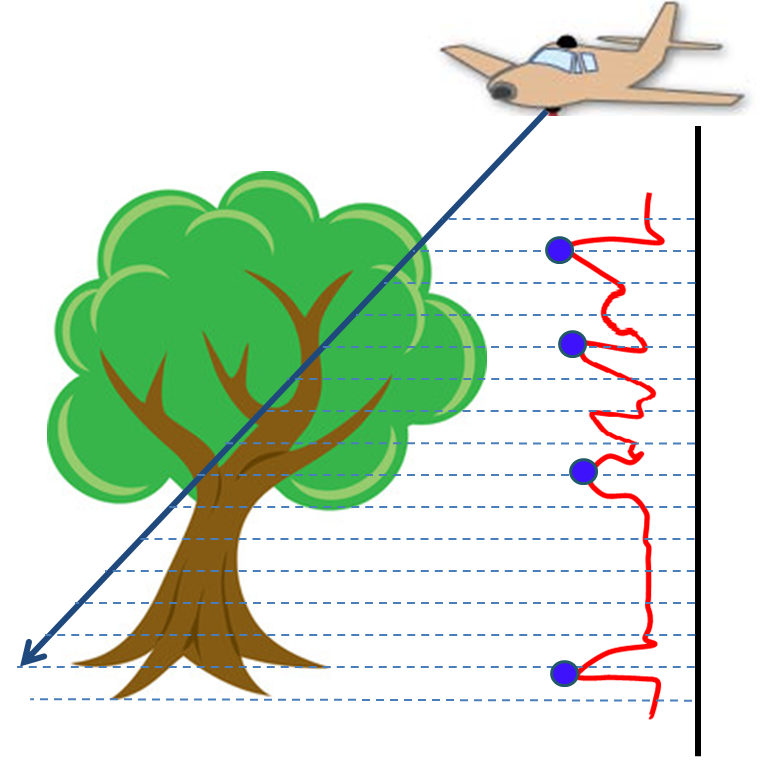
\includegraphics[width=.9\linewidth]{img/LiDAR_DiscretVsFW_fig}
  \caption{A Pulse: Discrete Vs Full-Waveform}
  \label{fig:ALS_flightline}
\end{subfigure}%
\begin{subfigure}{.5\textwidth}
  \centering
  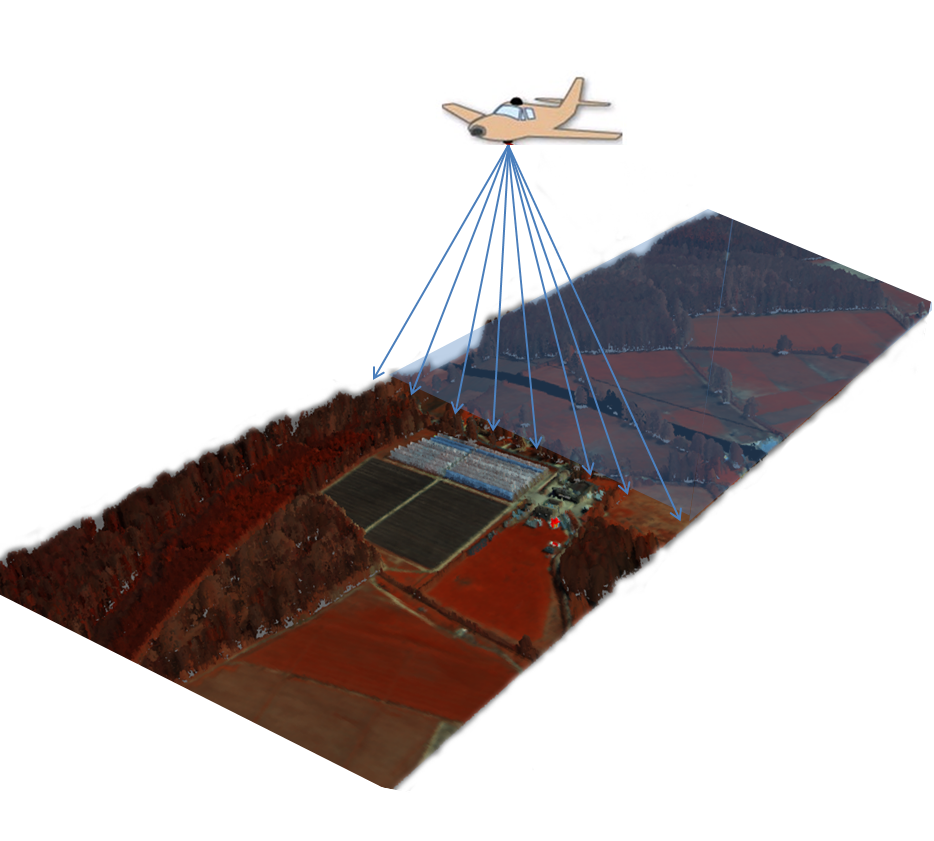
\includegraphics[width=\linewidth]{img/Flightline2}
  \caption{A Flightline}
  \label{fig:ALS_pulse}
\end{subfigure}
\caption{Airborne Laser Scanning System}
\label{fig:ALS_system}
\end{figure}
%	\footnotemark}
%	           	\footnotetext{Tree image was retrieved from http://images.clipartpanda.com/tree-clip-art-Kij4jKriq.jpeg on 7th o f June. The plane image was retrieved form http://gmv.cast.uark.edu/wp-content/uploads/2013/01/ALS\_scematic.jpg on the 6th of June} 




    \section{Airborne LiDAR systems: An in-depth Explanation}\label{sec:ALS}
     
        
    
    The ALS systems emit laser beams from a plane and collects information from the  returned laser intensity. When the beam hits an object (i.e. the forest canopy), then some of it bounces back while the rest penetrates through the tree branches. The laser beam continuous to break and partially return to the sensor until it reaches the ground. The LiDAR systems record information from the backscattered laser and by measuring its round trip time. 

     
     As mentioned at Section \ref{Background}, there are two types of LiDAR data, the discrete and the FW. The discrete LiDAR records a few peak laser returns, while the FW LiDAR system digitises and records the enitre backscattered signal into equally spaced time intervals (Figure \ref{fig:ALS_pulse}). The delivered data for the discrete LiDAR is a set of hit points, returns, which are associated with laser intensities. The position of every return is calculated by measuring the round trip time of the laser beam. The waveforms are attached to first returns of discrete LiDAR data and they are a list of intensities that correspond to the laser intensity returned over time. There is also an offset vector which defines the distance between each wave sample.
     
    Nevertheless, as shown at Figure \ref{fig:ALS_flightline}, the scanned data has a limited maximum width according to the flight height and the field of view scan angle. During processing the track of the plane is divided into easier to handle pieces (flightlines) and saved into separate binary files. In this project the LAS1.3 file format is used for both datasets. 
      
     
    \section{ Brief Explanation the LAS1.3 File Format} \label{sec:LAS1_3_specifications}
    
    \par There are a few LiDAR file formats but the LAS1.3 binary was the first format to contain FW data and it is the one used to store the data for both  New Forest and RedGum datasets. According to LAS1.3 file specifications \cite{LAS1.3specifications}, a .LAS file contains information about both discrete and FW LiDAR data and the waveform packets are attached to discrete returns and saved either internally at the end of the .LAS file or externally in a .WVS file. 
    
    \par As shown at (Figure \ref{fig:LAS1_3_fileFormat}) the .LAS file is divided into four sections and a brief explanation of each section is given here:
    \begin{enumerate}
    \item  The \textbf{Header} contains general information about the entire flightline. For example, it includes the scan angle used during the flight, whether the waveform packets are recorded internally or externally  and the number of \textbf{Variable Length Records} (VLR). 
    \item Regarding the \textbf{VLR}, the most important information given is the waveform packet descriptors that contain essential information on how to read the waveform packets (i.e. an ID, the number of wave samples and the size of each intensity in bits). 
    \item The \textbf{Point Data Records} are the discrete points and the waveforms are associated with first return discrete points. Each Point Data Record has a spatial location, an intensity and optionally a pointer to a waveform packet as well as the ID of the corresponding waveform packet descriptor. 
    \item The waveform packets is a list of intensities and they are either saved internally into the \textbf{Extended Variable Length Records} section of the .LAS file or inside an external .WVS file. Starting from the associated first return point, the spatial location of the waveform packet (wave sample intensity) are calculated by adding an offset defined in the associated Point Data Record. 
    \end{enumerate}  
    

	 \begin{figure}[!htbp]
           \centering
           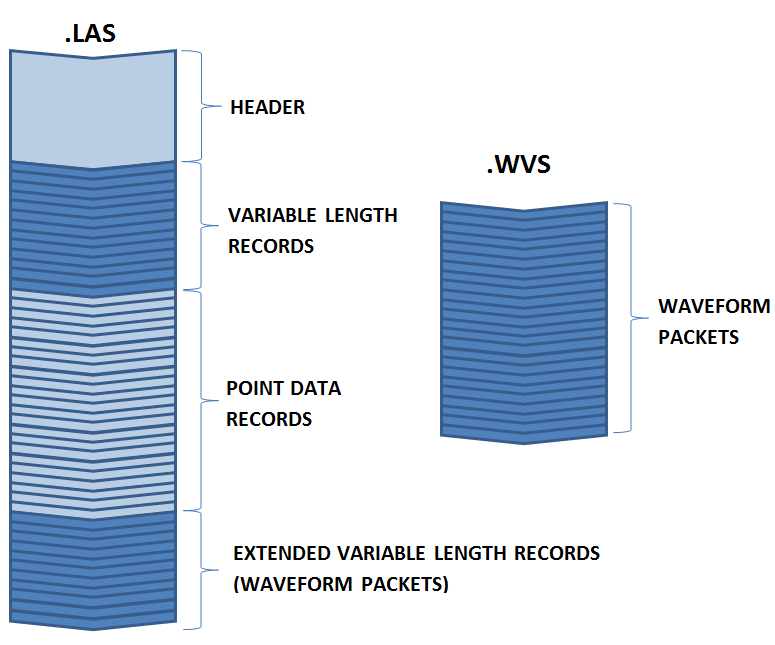
\includegraphics[width=\textwidth/3*2]{img/LAS1_3_fileFormat}
           \caption[Airborne LiDAR system]{}
           \label{fig:LAS1_3_fileFormat}
      \end{figure}

	\section{Leica Vs Trimble Instruments: Limitations, Differences and Advantages}\label{sec:LeicaVsTrimble}
	
	
	\par As shown in Figure \ref{fig:dataInstrumentsRelations}, the Leica ALS 50-II instrument was used to capture the LiDAR data of New Forest dataset and the Trimble AX60 for collecting the RedGum Forest FW LiDAR data. It is therefore important to clarify the differences, the limitations and the advantages of each instrument. 
	
	\par The Trimble performs at frequency 400kHz, while the Leica's maximum scanning frequency is 120kHz. Nevertheless, during experiments there were occasions when the Leica discarded every other waveform by exceeding its maximum scanning frequency \cite{Warren2012}. The New Forest dataset has been affected with this bug and on average 34.9(this is for one file I need to do it for the entire dataset)***\% of the saved pulses only contain discrete data. We should therefore be extremely careful when comparing Discrete with FW LiDAR data. At \cite{Sumnall2016}, it is stated that extra information, the echo-width, from the FW LiDAR data are relatively unimportant but the New Forest datasets were used for the comparison and there is no mention about the significantly less waveforms recorded in comparison to the discrete data.   
	
	\par Another problem with the Leica sysyem is the small range of intensities due to the number of bits used for recording them; the Leica system uses 8bits integers (0-255 range) while the Trimble uses 2bits integers (0-16385 range). For increased range and finer intensities, the Automatic Gain Controller (AGC) value was introduced. The AGC is an 8bit number that defines how the recorded intensity range is shifted across a wider range of intensities. The AGC value is adjusted according to the reflected laser intensity of the previous pulse and it therefore varies across a flightline. Consequently, the raw intensities are incomparable to each other and since the relation between AGC and the intensities is not linear, the range normalisation is complicated \cite{Lehner2011}\cite{Korpela2010}. In this thesis, the intensities of the Leica system are used as boolean values (whether something exist or not using a user-defined threshold) to quickly overcome that issue and focus on the major research objectives. Regarding the Trimble instrument, there is no AGC value because the intensities are saved into a 16bit integer and as long as the flight height is constant no normalisation is required. In a few words, the raw intensities recorded using the Leica system are not normalised and therefore not comparable to each other, while the intensities of the Trimble instrument are more meaningful. 
	
	\par Moreover the footprints of the laser on the ground depends on the scanning pattern of the instruments and the field of view. The sinusoidal scanning pattern of Leica system results into higher intensity of footprints at the edges of the flightline. The footprints of the Trimble instruments are more equally spaced because they are scanned using a rotating polygon. The problem of the uneven footprints of the Leica system is solved by normalisation during the voxelisation but the equally spaced footprints are more prone to aliasing when voxelised. Regarding the field of view, Leica has a wider field of view but in both cases big angles are avoided because otherwise data look deformed at edges of the flightlines. 
	
	\par Last but not least, the sensor of the Trimble instrument is a native full-waveform sensors and the discrete LiDAR are produced by extracting peak points at post-processing. Therefore the concept of extracting a denser point clouds using Gaussian decomposition \cite{Wanger2004} does not apply on data collected with those sensors. That was also proved by extracting peak points from Trimble FW LiDAR data using the pulseextract from LAStools ~\cite{LAStools}; the number of points extracted was exactly the same as the number of points saved into the associated discrete LiDAR files. Therefore Discrete data from the Trimble instrument are the same as FW LiDAR point cloud generated by echo decomposition and peak points extraction. 
	
	To sum up, the Trimble AX60 instrument is a newer sensor and therefore has less problems in comparison to the Leica ALS50-II instrument. Table \ref{tab:InstrumentsSpecs} summarises the differences between the two sensors. 
	
	\begin{table}[!htbp]
		\label{tab:InstrumentsSpecs}%
		\centering
		\begin{tabular}{|l||m{\textwidth/4}|m{\textwidth/4}|}
			\hline
			\textbf{Instrument Name:}	& \textbf{Leica ALS550-II}     & \textbf{Trimble Ax60  }    \\
			\hline\hline
			\textbf{Scanned Area} & New Forest, UK & RedGum, Australia \\
			\hline
			\textbf{Year of Introduction: }&Discrete LiDAR 2009 \& FW LiDAR 2010& 2013  \\
			\hline
			\textbf{Max Scan Frequency (kHz):} & 120 & 400  \\
			\hline
			\textbf{Recorded Intensity (bits):} & 8 & 16 \\
			\hline
			\textbf{AGC:} & Yes & No \\
			\hline
			\textbf{Scanning Pattern:} & Sinusoidal  & The footprints are more equally spaced on the ground \\			
			\hline
			\textbf{Max field of view (degrees):} & 75 & 60	\\
			\hline
		\end{tabular}%
		\caption{Specifications of the LiDAR instruments used}
	\end{table}
	


	\section{Hyperspectral Imagery}\label{sec:HyperspectralImages}
	\par Hyperspectral imagery has a positive impact in remote sensing because they contain information beyond human's visibility. The human eye receives light from the visual spectrum into three bands (red, green and blue). The hyperspectral sensors captures a larger spectrum and divides its light components into hundreds of bands, recording this way more information than a human eye can receive\cite{Smith2012}. 
	
	\par Nevertheless, raw airborne images  appear deformed because the pixel length varies across the flightline. NERC ARSF geo-corrects the data using the Airborne Processing Library (APL) \cite{Warren2014}. The processing levels are numbered. At 'level 3' the pixels are equally spaced and sized, but are slightly blurred. In this thesis, the 'level 1' data are used to preserve the highest possible quality. The 'level 1' data are non geo-corrected but they are associated with a file that defines the spatial location of each pixel. In practise, there are two files, the '.bil' and the '.igm'. The '.bil' file contains the hyperpsectral cube (Figure \ref{fig:hyperspectralCube}), all the pixel values at different wavelengths, and the .igm file gives the $x, y, z$ coordinates of each pixel.  
	
	\par The number of bands and the spectrum range captured depends on the hyperspectral sensor. The data from New Forest were collected using the following instruments:
	\begin{itemize}
		\item the Eagle, which captures the visible and near infra-red spectrum (400-970nm)
		\item the Haw, which covers short wave infra-red wavelengths(970-2450nm) 
	\end{itemize}
	Both sensors divide their spectrum range into 252 bands and each band is a 2D vector as shown in Figure \ref{fig:hyperspectralCube}).
	
	\begin{figure}[!htbp]
		\centering
		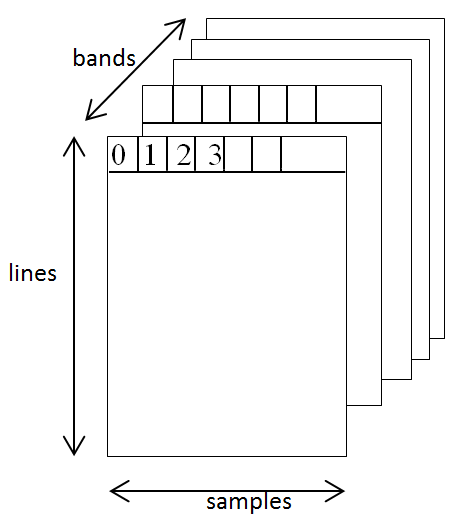
\includegraphics[width=\textwidth/5*2]{img/HI_bilFile}
		\caption[Hyperpsectral Cube]{This figure shows the order of the hyperspectral pixels saved into the the binary .bil file.}
		\label{fig:hyperspectralCube}
	\end{figure}
	
	By the way, the hyperpsectral images also come with a number of drawbacks. A few are mentioned here but since hyperpsectral imagery is not the main focused of the thesis there are not addressed:
	\begin{itemize}
		\item System faults sometimes occurs and the affected areas are masked out. This results into blank areas. 
		\item As a passive sensor, it is weather dependant and some areas are covered with clouds.
		\item Due to the high refraction of light at some wavelength, some bands are highly influenced by humidity (i.e. wavelength 1898.33).
	\end{itemize}
	
	To sum up, hyperpsectral images contain information beyond the visible and they are delivered into two file, one contains the hyperspectral cube and the other one the geo-locations of each pixel. In this project, they are used at chapter (Chapter \ref{Alignment}), where it is shown that the combination of Remote Sensing data confers better results for generating tree coverage maps. 
	
	
	
	
\end{document}